
%\begin{figure}[htbp]
%\begin{center}
%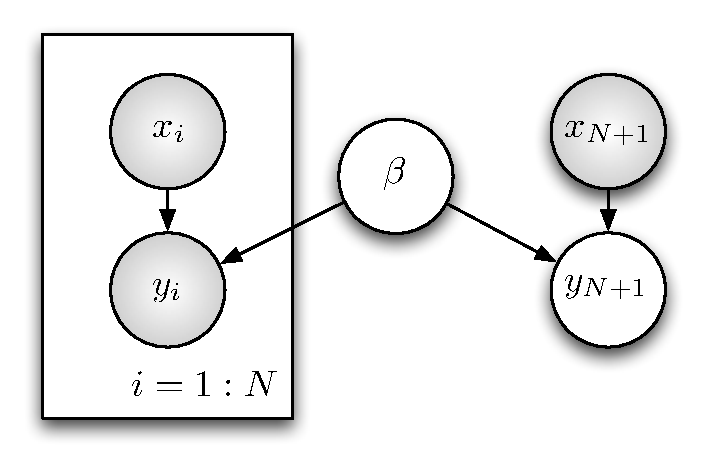
\includegraphics{Chapters/chapter1/probit_no_aux_vars}
%\caption{Probit model, no auxiliary variables}
%\label{fig:probit_no_aux_vars}
%\end{center}
%\end{figure}
%
%%
%%\begin{figure}[htbp]
%%\begin{center}
%%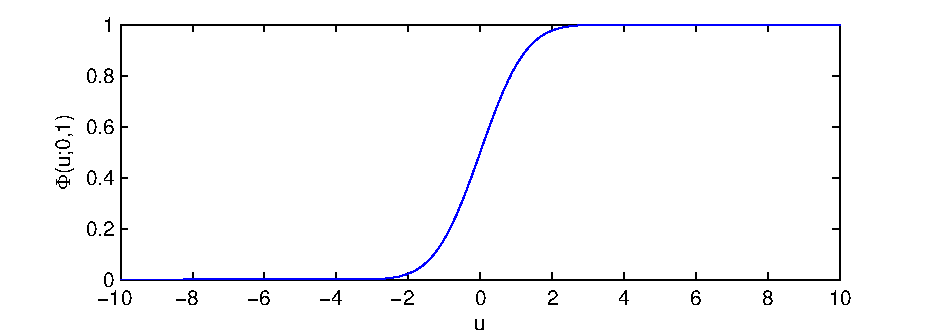
\includegraphics{Chapters/chapter1/cdf}
%%\caption{CDF of $N(0,1)$}
%%\label{fig:cdf}
%%\end{center}
%%\end{figure}
%
%\begin{figure}[htbp]
%\begin{center}
%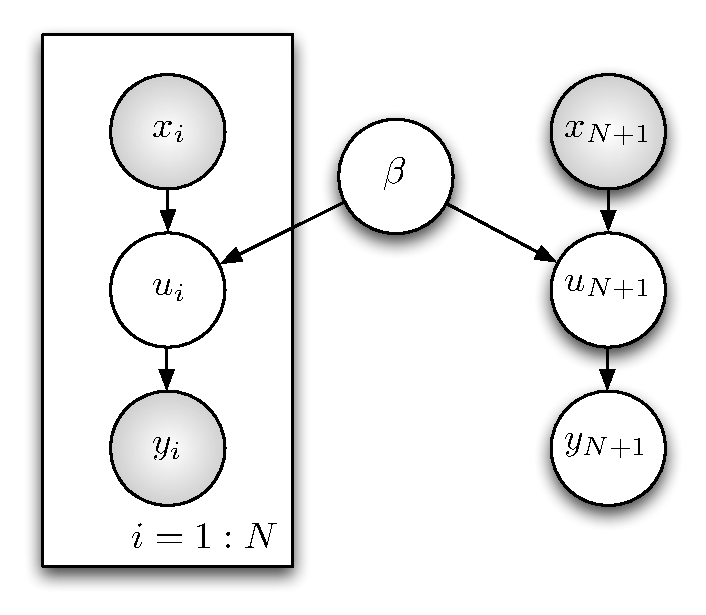
\includegraphics{Chapters/chapter1/probit}
%\caption{Probit model}
%\label{fig:probit}
%\end{center}
%\end{figure}




%For reasons that are somewhat obscure to me, statisticians tend to use probit regression for binary classification whereas machine learners tend to use logistic regression.  In a recent paper, my collaborators and I found it useful for computational purposes to use probit regression.  One can find many good primers on probit regression around the web, but, as we all know, there is almost always space for another.  
%
%Figure \ref{fig:cdf} is the cumulative distribution function (cdf) of a $N(0,1)$ distribution. 
%
For reasons that are somewhat obscure, statisticians tend to use probit regression for binary classification whereas machine learners tend to use logistic regression.
 The ``probit'' function is the inverse of the normal cumulative distribution function (cdf).    We denote the normal {\em cdf} function $\Phi(x;\mu,\sigma^2)$ with $\mu$ the mean, $\sigma^2$ the variance and $x$ the argument.

The range of the normal cdf is $(0,1)$ which means that it can be interpreted as a probability.  For instance, one can construct a generalized linear classification model (a ``probit regression model'') of the form 
\begin{equation}
P(y_i = 1) = \Phi(x_i^T\beta; 0, \sigma^2). \label{eqn:probit}
\end{equation}  Depending on convention (i.e. binary $y_i$ represented as $\{1,0\}$ or $\{1,-1\}$) then the probability of $y_i$ being labeled the opposite way is $P(y_i = -1)$ or $P(y_i = 0) = 1 - P(y_i=1).$  Here $x_i$ is a vector of covariates, $\beta$ is a vector of weights, and $y_i$ is a single, binary valued response.  As always, the close relationship between regression and classification are in full display here : probit regression is a ``generalized linear {\em regression} model'' as well as a ``binary classifier.''

%Figure \ref{fig:probit_no_aux_vars} shows the graphical model for probit regression (minus any priors on the regression weights $\beta$).   
 In this model we would like to use labeled training data, $\{x_i, y_i\}_{i=1}^N$ to ``learn'' the value of $\beta$ and then to use this value to predict the value of $y_{N+1} | x_{N+1}, \beta.$  If we are being Bayesian about our inference here what we really mean is that we will average over the posterior distribution of $\beta$ when making predictions.  This means that we want to draw samples from the posterior distribution of $\beta | \{x_i, y_i\}_{i=1}^N$.  To to this efficiently one can introduce a set of auxiliary variables $\{u_i\}_{i=1}^N$.  
 %In this note we will demonstrate that the model in  Figure \ref{fig:probit} is the same as the model in Figure \ref{fig:probit_no_aux_vars}  when the $u_i$'s are marginalized out and will suggest that inference in the former is computationally easier.  

By auxiliary variable we mean that such variables will be used as an intermediary for purposes of efficiency but will otherwise be uninteresting.    They are variables introduced into a model in order to make inference easier but whose existence does not change the distribution of interest.  Auxiliary variables for slice sampling are one particularly clever use of auxiliary variables.  The auxiliary variable trick in probit regression is another.

For the purposes of exposition, forget about the $i$ index for a bit and focus on a single instance $y$, $x$, and $u$.  The argument we make will hold for all by simply reintroducing subscripts.  

To start, let's propose a factorized joint distribution for these quantities

\begin{equation}
P(y,x,u) = P(y|u)P(u|x,\beta) \label{eqn:joint}
\end{equation}

Straight away, one can see why this auxiliary variable scheme works.  By the law of total probability we have
\begin{equation}
P(y,x) = \int P(y,x,u)du= \int P(y|u)P(u|x,\beta)du.  \label{eqn:joint_marginalized}
\end{equation}
So, if by some means we generate $S$ samples $\{u^{(s)},y^{(s)},x^{(s)}\}_{s=1}^S \sim P(y,x,u)$ we know that marginalizing $u$ out (i.e.~disregarding its value) we get samples $\{y^{(s)},x^{(s)}\}_{s=1}^S \sim P(y,x).$  %Equation  \ref{eqn:joint_marginalized} 
%\begin{eqnarray}
%y_i &\sim& \Phi(x_i^T\beta; 0, 1)
%\end{eqnarray}

We haven't specified the most important part of the auxiliary variable sampling scheme yet, namely, what $P(y|u)$ and what $P(u|x,\beta)$ are.   Let's try $y = \mbox{sign}(u)$ and $u \sim N(x^T\beta,\sigma^2).$  These choices are nice in a particular way.  First let's verify that the marginalization of $u$ out of this model results in the model specification in Equation \ref{eqn:probit}.

\begin{eqnarray*}
P(y=1|x,\beta) &=&  \int P(y=1|u)P(u|x,\beta)du\\
&=& \int \mathbb{I}(u>0)N(u;x^T\beta,\sigma^2) du \\
&=& \int_0^\infty N(u;x^T\beta,\sigma^2) du \\
&=& 1 - \Phi(0; x^T\beta,\sigma^2) \\ 
&=& \Phi(x^T\beta; 0, \sigma^2)
\end{eqnarray*}
where the last line comes from the fact that for symmetric distributions like the normal distribution, 
$\Phi(x^T\beta; 0, \sigma^2) = 1 - \Phi(-x^T\beta; 0, \sigma^2)$ and the mean of a normal cdf can be translated arbitrarily, i.e. $\Phi(-x^T\beta; 0, \sigma^2) = \Phi(0;x^T\beta, \sigma^2)$ (which comes from adding the offset $x^T\beta$ to the cdf argument and mean).  

Having established the fact that for a particular sort of auxiliary variable choice, we get the same probit model as we wanted, why is this choice nice?

Well, it comes down to sampling $\beta$ and $u$ and $y$.  Generally, sampling $\beta$ in the model without auxiliary variables will require hybrid Monte Carlo (HMC) or Metropolis Hastings of some sort.  Gibbs sampling often comes with substantial benefits.  By making this choice of auxiliary variable the conditional distribution of $u_i$ given everything else is proportional to a truncated Normal distribution, a distribution that is, by nature of its commonness, relatively straightforward to sample from.  The big benefit, though, acrues from the posterior form for sampling $\beta$.  With the $u$'s ``observed'' (as they would be in a Gibbs sampler), the posterior distribution of $\beta$ (for typical choices of prior) is precisely the same as that for linear regression, perhaps the most well studied model in statistics.  In that case, sampling $\beta$ from its posterior distribution is quite simple usually; certainly more so that sampling $\beta$ without the $u$ auxiliary variables.

The extension to the multivariate HSLDA setting is straightforward and follows this line of reasoning precisely.  An extended discussion of the techniques suggested here and the multivariate generalization can be found in \cite{gelmanbda04}.

